\documentclass[10pt,a4paper]{report}
% Paquetes
\usepackage[utf8]{inputenc}
% Para cocina
\usepackage{xcookybooky}
% Idioma
\usepackage[english, spanish]{babel}
% Indice, o urls
\usepackage[bookmarks = true, colorlinks=true, linkcolor = black, citecolor = black, menucolor = black, urlcolor = blue]{hyperref}
% Paquetes de imagenes
\usepackage{graphicx}
\usepackage{wrapfig}
% Ruta de imágenes
\graphicspath{ {pix/} }
% Lenguaje
\selectlanguage{spanish}
% Interlineado
\usepackage{setspace}
% Para paginaciones
\usepackage{fancyhdr}
% Limpia cabecera y pie de página
\fancyhead{}
\fancyfoot{}
% Setea número hacia el lado derecho del pie de página
\fancyfoot[R]{\thepage}
% Configura xcookybooky
\setHeadlines{
    inghead = Ingredientes,
    prephead = Preparación,
    hinthead = Tips
}

% Título
\title{Recopilación De Recetas Familiares}
\author{El Happy}

% Imagen de fondo de Borrador
%\usepackage{eso-pic} % imagen de fondo
%\newcommand\imgFondo{%
%   \put(0,0){%
%     \parbox[b][\paperheight]{\paperwidth}{%
%       \vfill
%       \centering
%       
\includegraphics[width=\paperwidth,height=\paperheight,%
%       keepaspectratio]{borrador}%
%       \vfill
%		}
%	}
%}

% Inicio del documento
\begin{document}
%----------------------------------------------------------------------------------------
%	Portada
%----------------------------------------------------------------------------------------

\begingroup
\thispagestyle{empty}
\AddToShipoutPicture*{\put(0,0){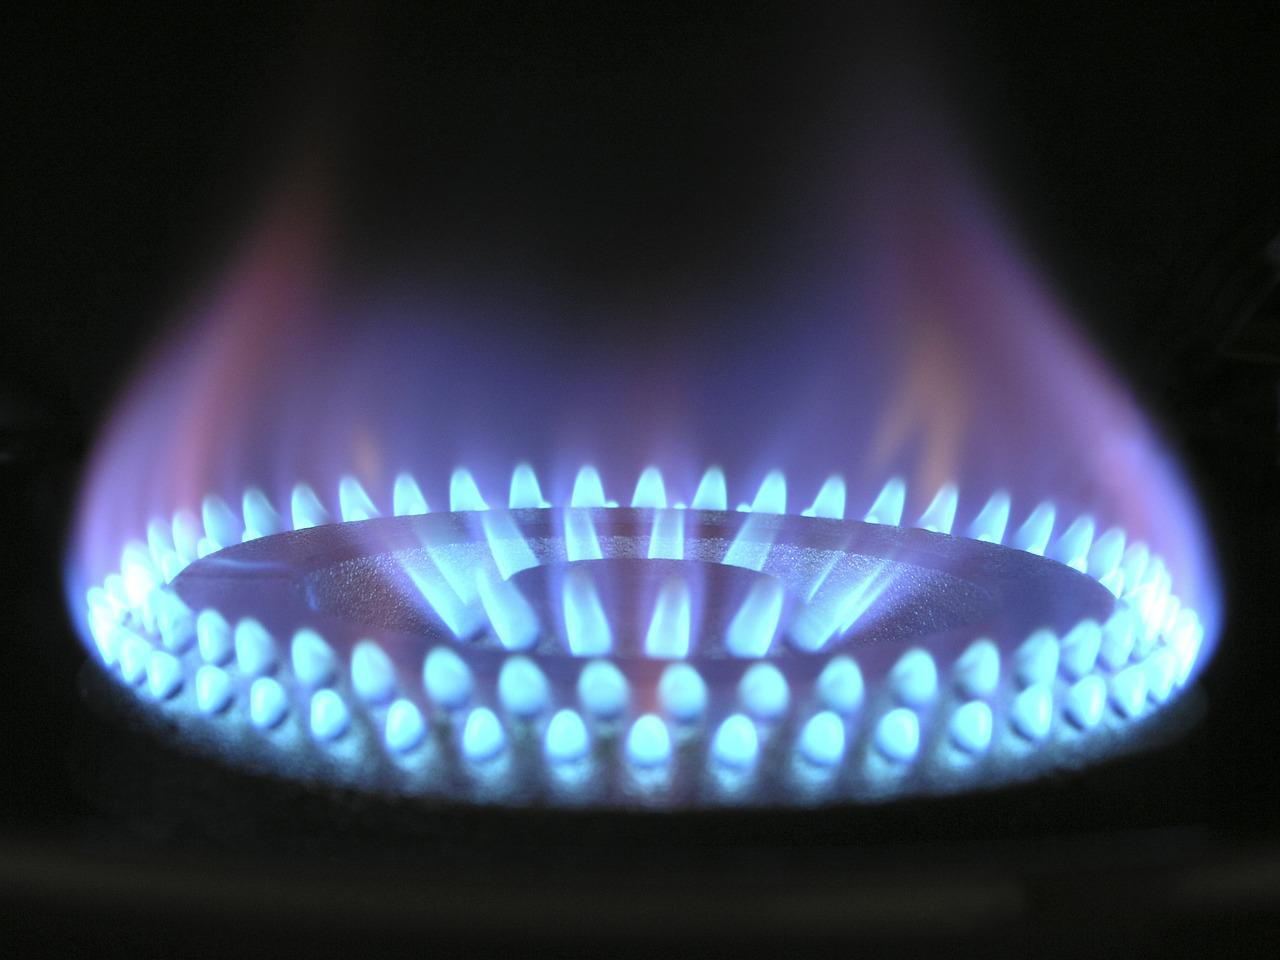
\includegraphics[scale=1]{fuego}}} % Image background
\centering
\vspace*{5cm}
\par\normalfont\fontsize{35}{35}\sffamily\selectfont
{\LARGE Recopilación De Recetas Familiares}\par % Book title
\vspace*{1cm}
{\Huge El Happy}\par % Author name
\endgroup

%----------------------------------------------------------------------------------------
%	Dedicatoria, Derechos de autor... 
%----------------------------------------------------------------------------------------

\newpage
% Imagen de fondo de borrador
%\AddToShipoutPicture{\imgFondo}
~\vfill
\thispagestyle{empty}

\noindent \textsc{A mi esposa:}\\

\noindent Por su compañía, por sus ocurrencias y sus singulares ideas de probar cosas nuevas, algunas plasmadas en este libro...\\

\noindent A mi madre: Es la mejor cosa que uno tiene en este mundo...\\ 

\noindent Finalmente, a mi padre, a quien le rindo homenaje en este libro...

\noindent \textsc{https://fotosycaptura.cl}\\ % URL

\noindent \textit{Escrito por Xavier Fuentes, usando \LaTeX, Junio 2022}

%----------------------------------------------------------------------------------------
%	Indice General
%----------------------------------------------------------------------------------------

\newpage
\tableofcontents
\newpage

%----------------------------------------------------------------------------------------
%	Introducción
%----------------------------------------------------------------------------------------

\chapter*{Introducción}
\thispagestyle{empty}
\spacing{1.5}

\begin{wrapfigure}{r}{0.25\textwidth}
	\scalebox{0.5}{
		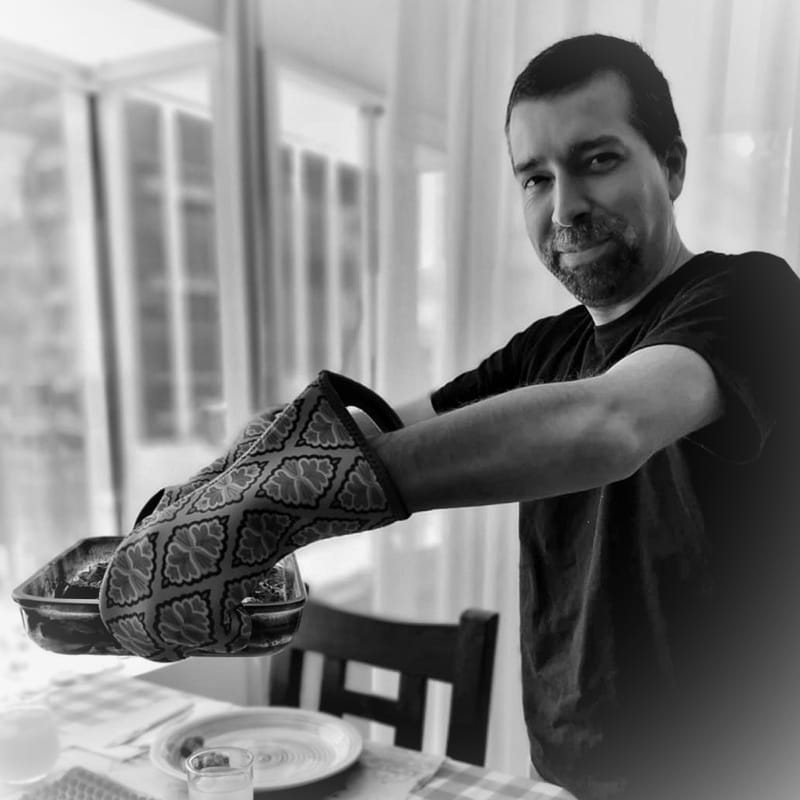
\includegraphics[width=0.48\textwidth]{autor}
	}
\end{wrapfigure} 

Este libro es un pequeño tributo a la memoria de las recetas de cocina de la familia, al sabor, al disfrute de los alimentos pero más que todo eso a la compañía o reunión de familia, amigos y seres queridos, que alguno de ellos
ya no están. 

En la vida cotidiana, de pequeños hemos visto a alguno de nuestros padres que dedican tiempo en la cocina y realizan algunos platos que más que alguna ocasión han sido el deleite nuestro como hijos. En ocasiones, habían desayunos, almuerzos o comidas que en sí eran especiales, eran diferentes del menú diario por algún tipo de evento, otras en cambio, eran comidas que quizás en algún momento no queríamos como niños, pero que ahora como adulto, apreciamos el detalle, el contexto, y cada uno de esos platos puede evocar un hermoso recuerdo.

A lo largo de la vida, las recetas se han transmitido de generación en generación por diversos medios, algunos han tenido la dicha de aprender directamente de sus familiares, otros en cambio por el echo de mirar a otros, y otros simplemente al comer, y ver los elementos en la comida, y comenzar con esa curiosidad de cómo es que conforman el plato en sí. 

No quiero extenderme mucho más pues esto no es un estudio científico o algún tipo de documento de análisis,  simplemente es una recopilación de las recetas típicas del hogar en el que viví, así como también algunas otras que he aprendido a lo largo de la vida, recetas tradicionales chilenas, alguna cosa extranjera, y que son relativamente fáciles de hacer en casa.

Porque en la vida, en ocasiones, es grato darse tiempo a uno mismo en compañía con los suyos, y qué mejor momento que en un almuerzo, una once, una cena, o incluso un desayuno, y compartir momentos, vivencias que nos llenarán el alma y nuestros recuerdos para nuestras memorias en la vejez...


\newpage
\singlespacing 
% Se setean encabecados de página
\lhead{Recopilación De Recetas Familiares}
\rhead{El Happy}

%----------------------------------------------------------------------------------------
%	Recetas
%----------------------------------------------------------------------------------------

% Recetas
\chapter*{Cremas o Salsas}
\addcontentsline{toc}{chapter}{Cremas O Salsas}
% Crema o salsa de rocoto
\newpage
\thispagestyle{empty}
\begin{recipe}[source={Lizz}]{Crema De Rocoto}
\introduction{
La crema de rocoto es una salsa medianamente picante que sirve para acompañar diveros platos o para comer con galletas. Supe de su existencia cuando salí con Lizz a cenar a restoranes peruanos.
}
\ingredients{
    \unit[170]{gr} & de leche evaporada \\
    \unit[60]{gr} & de queso Fresco \\
    1 & Rocoto \\
    1 & Diente de Ajo \\
    4 & galletas de soda \\
    1 & cucharadita de sal \\
    1 & cucharada de aceite \\
}
\preparation{
    \begin{enumerate}
        \item Agregar todos los ingredientes a una licuadora.
        \item Procesar por unos 4 o 5 minutos.
        \item Ya está listo para servir.
    \end{enumerate}
}
\end{recipe}
%Salsa asado
\newpage
\thispagestyle{empty}
\begin{recipe}[source={Youtube},
preparationtime={\unit[2-5]{Minutos}}
]{Salsa Para Asados}
    \introduction{
        Esta preparación de salsa para asado la vi en un canal de youtube en sus días, me pareció interesante y después de probarla me gustó.
    }
    \ingredients{
        2 & cucharaditas de te de Oregano \\
        1 & cucharadita de te de aji de color \\
        1/2 & cucharadita de te de comino \\
        & Vinagre \\
        & Aceite de Oliva
    }
    \preparation{
        \begin{enumerate}
            \item Mezclar todos los ingredientes en un frasco.
            \item Aplicar con una brocha en la carne que vaya a asar.
        \end{enumerate}
    }
\end{recipe}


\chapter*{Platos principales}
\addcontentsline{toc}{chapter}{Platos Principales}
% Asado a la cacerola
\newpage
%\thispagestyle{empty}
\begin{recipe}[source={El papá},
portion={4-6 porciones},
preparationtime={\unit[2]{Horas}}
]{Asado A La Cacerola}
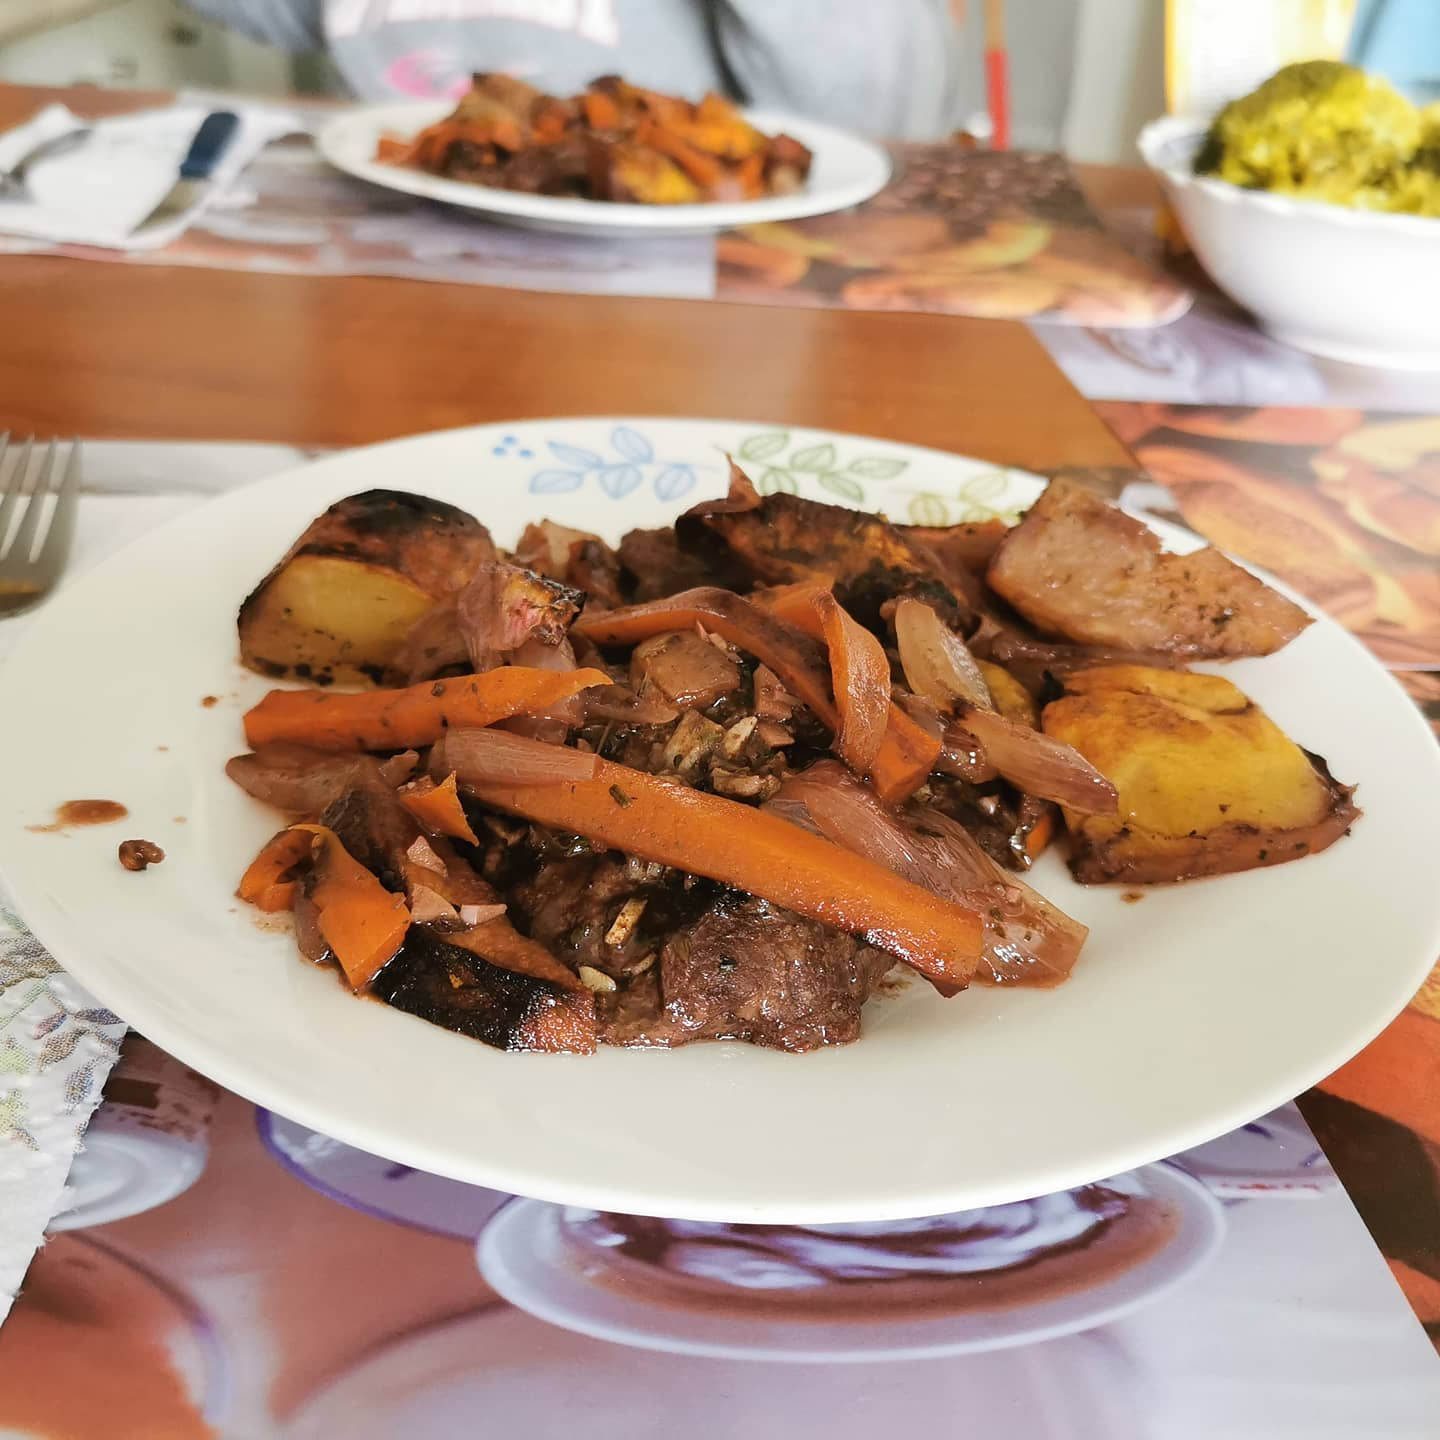
\includegraphics[width=0.25\textwidth]{asado-cacerola}
\introduction{
Esta es una receta muy añorada por mi familia. Era una de las especialidades de mi padre.
}
\ingredients{
    \unit[2]{Kg} & de carne de punta ganso \\
    2 & Cebollas cortadas en 4 \\
    2 & Manzanas cortadas en 4 \\
    3 & dientes de ajo picados \\
    & Orégano a gusto \\
    5 & papas \\
    2 & zanahorias cortadas en tiras finas a lo largo \\
    \unit[150]{gr} & Vinagre \\
    1 & copa de vino tinto \\
      & Aceite de oliva \\
      & Sal \\
      & Pimienta
}
\preparation{
    \begin{enumerate}
        \item Adobar la carne con los aliños y dejarla macerar al menos media hora como mínimo.
        \item Pre calentar el horno a 180 grados por 5 minutos.
        \item En una fuente para horno, meter la carne adobada con los aliños, la cebolla, la manzana, la zanahoria, las papas y finalmente la copa de vino.
        \item Meter la bandeja al horno y dejar cocinar por aproximadamente 2 horas.
        \item Retirar y servir. 
    \end{enumerate}
}
\hint{
	Se puede acompañar con arroz o ensalada.
}
\end{recipe}
\newpage
\thispagestyle{empty}
\begin{recipe}[source={Propia},
portion={4-5 porciones},
preparationtime={\unit[4]{h}\unit[15]{m}}
]{Costillar Al Horno}
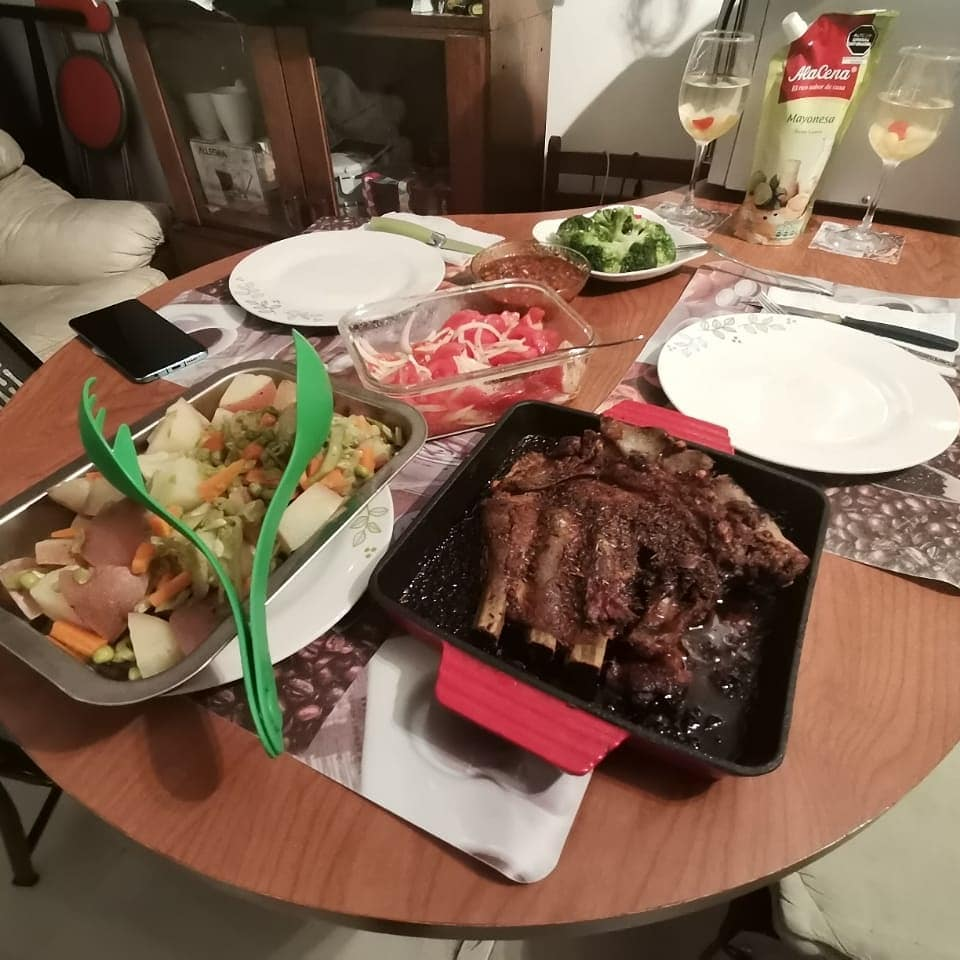
\includegraphics[width=0.25\textwidth]{costillar}
\introduction{
Esta es una receta propia. Los huesos salen solos
}
\ingredients{
    1 & costillar de cerdo \\
    2 & cucharadas de vinagre tinto \\
    & Sal a gusto \\
    & Pimienta molida a gusto \\
    & Comino a gusto \\
    & Orégano a gusto \\
    & Paprika o pimentón dulce a gusto \\
    1 & cucharada de aceite de oliva
}
\preparation{
    \begin{enumerate}
        \item Enbardunar las costillas con los aliños y dejar macerar.
        \item Tapar con film de aluminio y meter al horno pre calentado.
        \item Cocinar por una hora al horno. 
        \item Transcurrida la hora, apagar el horno y dejar enfriar en el mismo horno por 3 horas más.
        \item Quitar papel de aluminio.
        \item Pincelar con la salsa y calentar otra vez por 15 min.
    \end{enumerate}
}
\end{recipe}
% Ensalada sunomono
\newpage
\begin{recipe}[source={Adaptación propia},
portion={2-4 porciones},
preparationtime={\unit[20]{Minutos}}
]{Ensalada Sunomono}
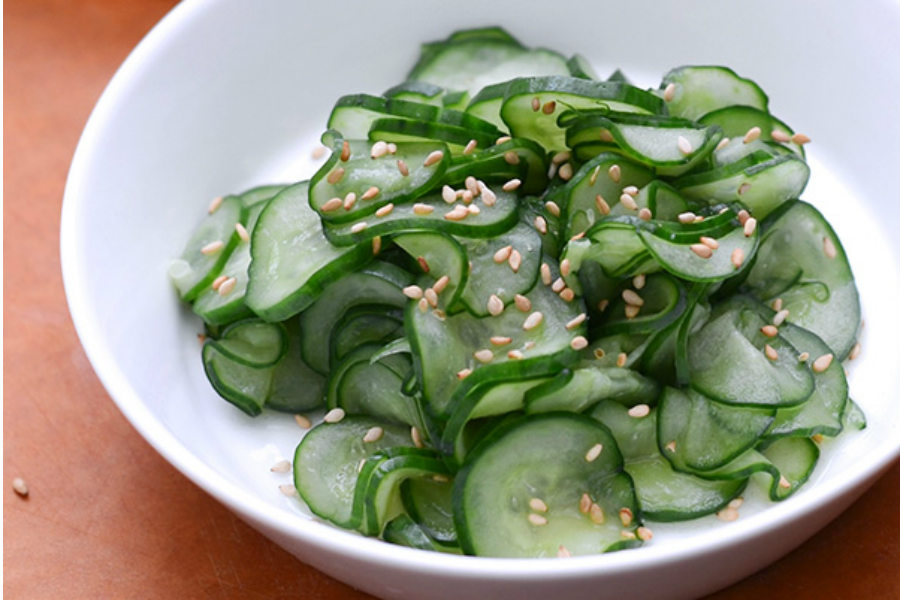
\includegraphics[width=0.25\textwidth]{sunomono}
\introduction{
Una receta que pillé en algún video de youtube. Me gustó su simplesa y lo rico que es
}
\ingredients{
    2 & pepinos \\
    1/2 & cucharada de sésamo \\
    1 & cucharadita de sal \\
    4 & cucharadas de vinagre de arroz \\
    1/2 & cucharada de salsa de soja \\
    2 & cucharadas de azúcar 
}
\preparation{
    \begin{enumerate}
        \item Cortar en láminas delgadas los pepinos y lavar con agua con sal unos 10 minutos.
        \item Escurrir el agua y comenzar a aliñar, integrando los demás ingredientes.
        \item Una vez revuelto, reservar en el refrigador al menos una media hora antes de servir.
    \end{enumerate}
}
\end{recipe}
% Lentejas
\newpage
\thispagestyle{empty}
\begin{recipe}[
source={La Mami y adaptación Propia}, 
portion={4-5 porciones},
preparationtime={\unit[1]{Hora}}
]
{Lentejas}
\introduction{
Me gustan mucho las lentejas, y sobre todo hecho sopa. La receta original corresponde a la de mi mami, pero la adapté a mi gusto particular. Esta preparación está pensada para olla a presión.
}
\ingredients{
    1 & taza de lentejas ya remojadas el día anterior \\
    1/2 & taza de arroz \\
	1 & zanahoria picada en cubitos pequeños \\
	3 & dientes de ajo picados finamente \\
	1 & cebolla picada a cuadritos finamente \\
	2 & Longaniza o  varias longanicillas \\
	& Sal a gusto \\
	& Orégano a gusto \\
	& Pimienta a gusto \\
	& Ají de color a gusto \\
	& Comino a gusto \\
	1 & cucharada de salsa de soja
}
\preparation{
	\begin{enumerate}
		\item En la olla a presión, agregue un poco de aceite de oliva.
		\item Corte las longanizas o longanicillas y comience a sellar en la olla.
		\item Prepare el sofrito en la olla agregando el ajo, cebolla, especias varias.
		\item Cuando el sofrito esté listo, agregue el arroz y revuelva durante al menos unos 2 minutos mínimo para granear el arroz.
		\item Agregue 3 tazas de agua.
		\item Agregue las lentejas.
		\item Agregue la salsa de soja y revuelva un poco.
		\item Tape la olla y deje cocinar por 25 minutos aproximadamente.
		\item Apague el fuego y deje enfriar la olla a presión.
	\end{enumerate}
}
\hint{
	Puede agregar un huevo duro para acompañar las lentejas en el centro del plato.
}
\end{recipe}
% Pizza casera
\newpage
\begin{recipe}[source={La Mami},
portion={2-6 personas},
preparationtime={\unit[1]{Hora}}
]{Pizza Casera}
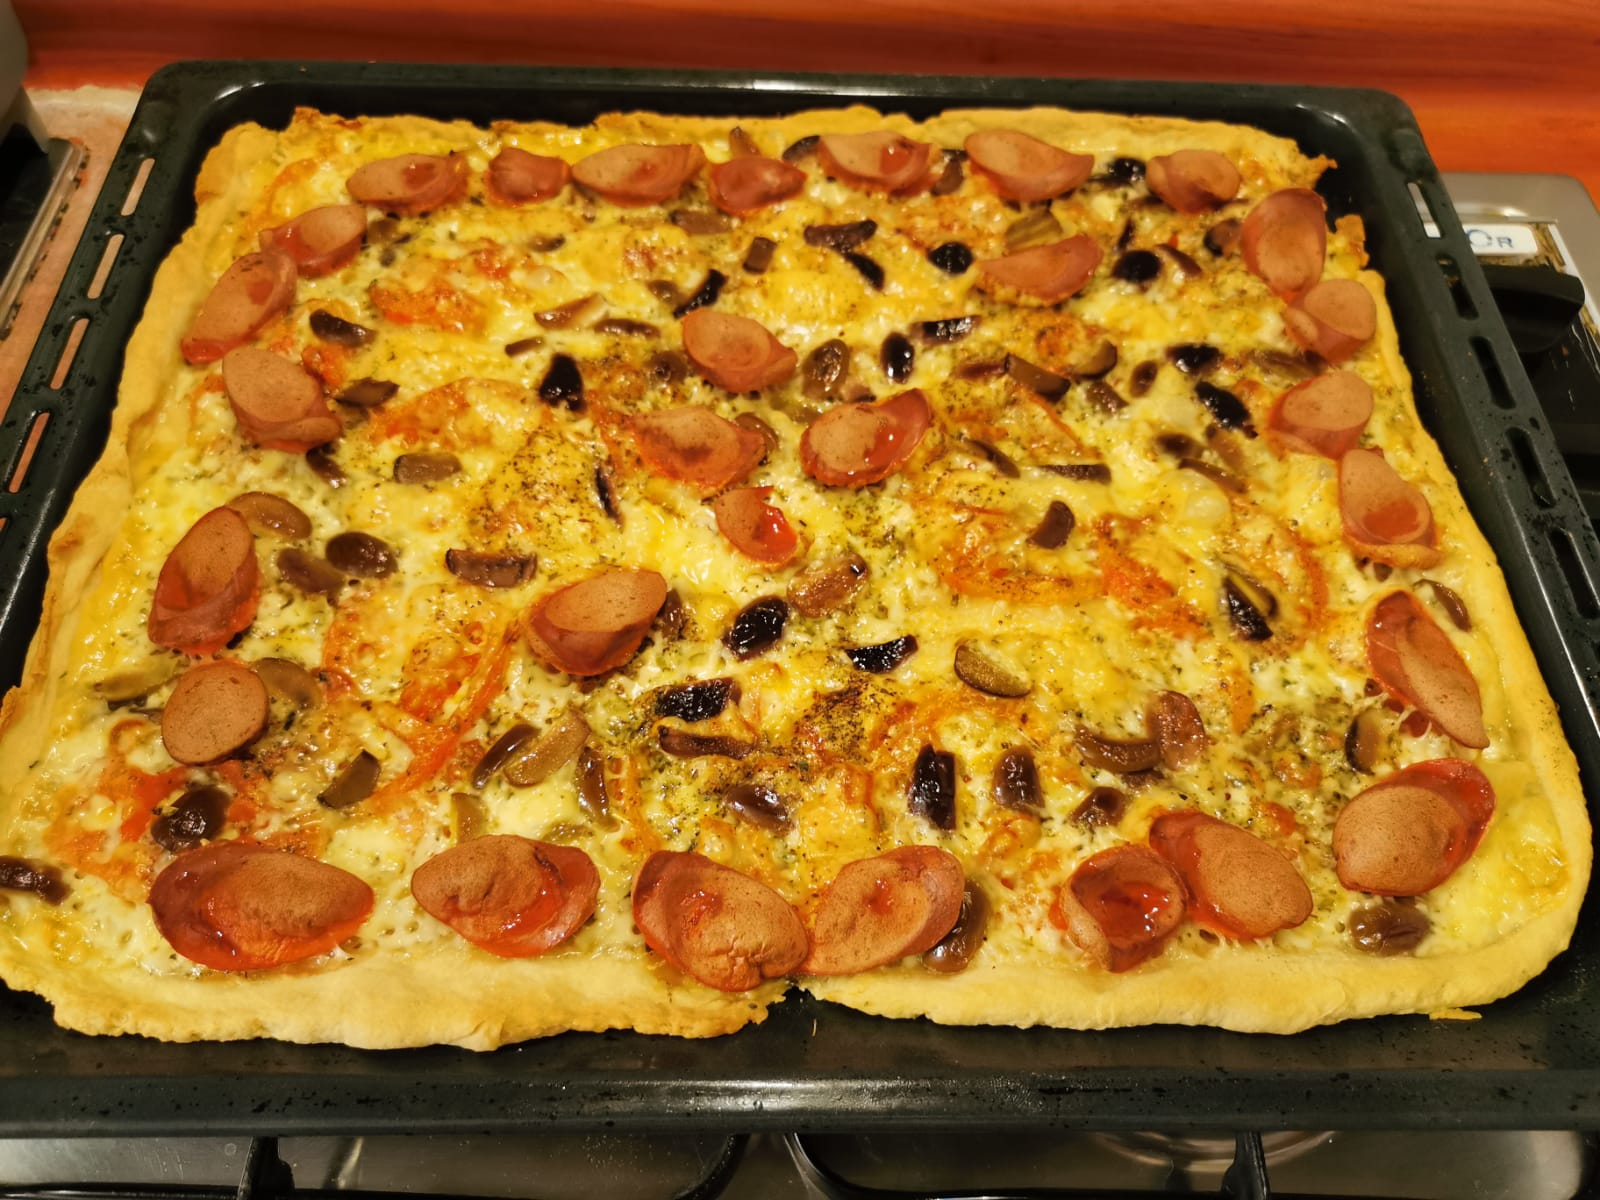
\includegraphics[width=0.25\textwidth]{pizza}
\introduction{
A quién no le gusta la pizza. Siempre son bienvenidas en cualquier momento y hora.
}
\ingredients{
	& \textbf{Para la masa:} \\
    4 & tazas de harina \\
    1 & cucharada de polvos de hornear \\
    1 & cucharadita de sal \\
    2 & cucharadas de aceite de oliva \\
    1 & taza de agua tibia o leche \\
    & \textbf{Para el acompañamiento:} \\
    2 & tomates cortados en rodajas finas \\
    \unit[500]{gr} & de queso laminado \\
    \unit[250]{gr} & de aceitunas \\
    \unit[100]{gr} & de salame \\
    & Orégano a gusto
}
\preparation{
    \begin{enumerate}
        \item Preparar la masa en un bol integrando la harina, la sal, el aceite, los polvos de hornear y poco a poco el agua.
        \item Pre calentar el horno por 5 minutos a 180 grados con calor arriba y abajo.
        \item Estirar la masa en la bandeja previamente aceitada.
        \item Colocar el tomate, el queso, el orégano, el salame y las aceitunas.
        \item Meter la bandeja al horno y cocinar por aproximadamente unos 30-40 minutos o hasta que los bordes de la masa estén dorados.
        \item Retirar y servir.
    \end{enumerate}
}
\hint{
	Puedes echar un poco de merquén si te gusta que tenga un condimento picante.
}

\end{recipe}
% Zapallitos Italianos Rellenos
\newpage
\thispagestyle{empty}
\begin{recipe}[source={La Mami y Youtube},
portion={6 porciones},
preparationtime={\unit[1]{Hora}}
]{Zapallitos Italianos Rellenos}
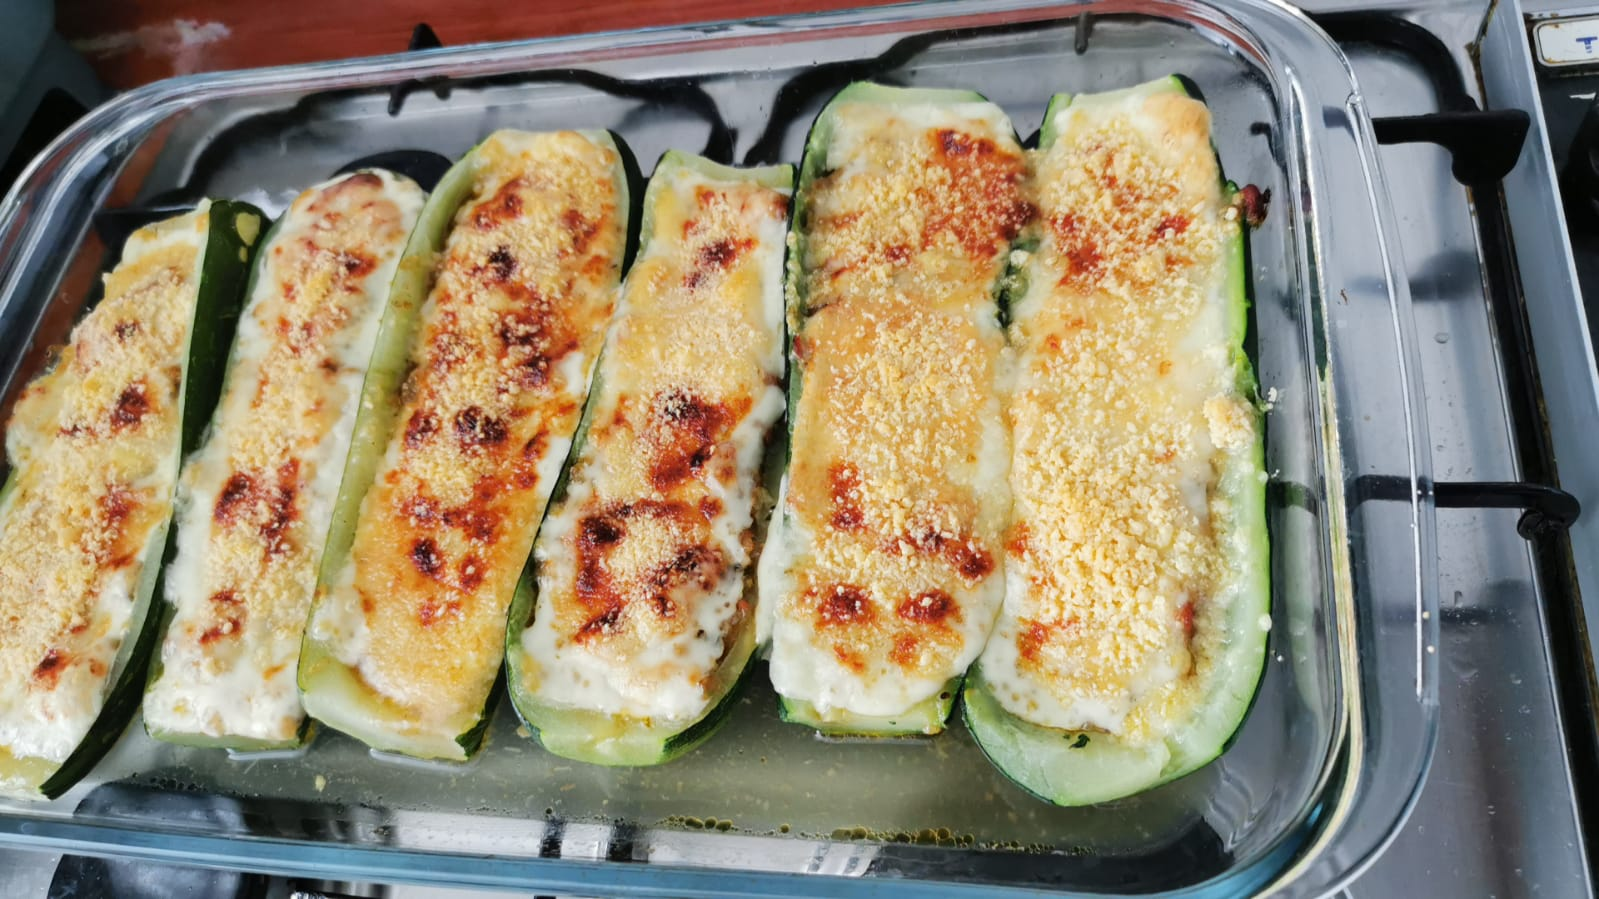
\includegraphics[width=0.25\textwidth]{zapallos-italianos}
	\introduction{
		Los zapallos italianos son una receta típica de la familia. Son muy ricos para comer solos, o acompañándolos con algún arroz o ensalada.
	}
	\ingredients{
		\unit[250]{gr} & posta molida de vacuno o cualquier corte magro \\
		3 & zapallos Italianos \\
		2 & cucharadas de aceite de oliva \\
		1 & taza de cebolla picada finamente en cuadraditos \\
		3 & dientes de ajo \\
		1 & cucharada de paprika o ají de color \\
		1 & cucharada de orégano fresco \\
		& Sal a gusto \\
		& Queso rallado
	}
	\preparation{
		\begin{enumerate}
			\item Cortar los zapallos italianos a lo largo a la mitad.
			\item Rascar los zapallos italianos por dentro de tal manera de ir dejando una
			      especie de canal por dentro y extraer el centro. Para esto se puede valer de
			      una cuchara.
			\item Cocer las mitades ya partidas y rascadas 10 minutos en agua hirviendo con sal.
			\item Para el relleno, en una olla se prepara un sofrito echando un poco del aceite
			      con el ajo picándolo finamente y agregando la cebolla, el orégano y finalmente
			      el relleno extraído de los zapallos, un poco de sal y revolviendo a fuego suave
			      entre 15 y 20 minutos.
			\item Escurrir los zapallos y extraer el relleno y colocar en una fuente para horno.
			\item Precalentar el horno a 180 grados con calor arriba y abajo durante 5 minutos.
			\item En la fuente colocar los zapallos y rellenar con el relleno preparado,
			      posteriormente decorar con el queso rallado y meter la fuente al horno hasta
			      que el queso quede gratinado por aproximadamente 15 minutos.
			\item retirar del horno y servir.
		\end{enumerate}
	}
\end{recipe}

% Postres
\chapter*{Postres}
\addcontentsline{toc}{chapter}{Postres}
% Almibar de Canela
\newpage
%\thispagestyle{empty}
\begin{recipe}[source={Charlie Good}]{Almibar De Canela}
\introduction{
Esta receta me la dio un compañero de trabajo, es especial para algunos tipos de cócteles o tragos como por ejemplo el pisco sour.
}
\ingredients{
    1 & taza de azúcar \\
    1 & taza de agua \\
    3 & trozos de canela en ramas
}
\preparation{
    \begin{enumerate}
        \item Verter el azúcar en una olla o sartén, junto con el agua y la canela.
        \item Poner a fuego fuerte y revolver de manera constante hasta que hierva.
        \item Una vez que hierva, dejar el fuego al mínimo y revolver de vez en cuando por al menos unos 15 minutos.
        \item Luego de ello, poner en un recipiente de vidrio y guardar y tapar. 
        \item No refrigerar. 
        \item Tiempo de máximo uso en el frasco 3 semanas.
    \end{enumerate}
}
\end{recipe}
% Bizcocho
\newpage
%\thispagestyle{empty}
\begin{recipe}[source={Esbieta},
preparationtime={\unit[1]{Horas} \unit[25]{Minutos}}
]{Bizcocho Para Torta}
\introduction{
Siempre pensé que el bizcocho para torta no debería de separarse la clara de las yemas para ir preparando, y encontré esta receta que es más antigua y funciona muy bien
}
\ingredients{
	7 & huevos \\
    \unit[210]{gr} & de harina \\
    \unit[210]{gr} & de azúcar \\
    1 & cucharadita de sal \\
    1 & ralladura de limón
}
\preparation{
    \begin{enumerate}
        \item Cascar los huevos en un bol, agregar el azúcar y proceder a mojar el azúcar con los huevos para que no salga volando al batir.
        \item En otro bol, tamizar la harina.
        \item Batir fuertemente por aproximadamente entre 12 a 15 minutos. Sabrá cuando está montada cuando al trazar una línea, ésta no desaparece después de 8 conteos. Desde este punto, se puede mezclar cuidadosamente con la harina.
        \item Con movimientos envolventes se debe de mezclar la harina con la mezcla cuidadosamente.
        \item Precalentar el horno por 10 minutos a 170 grados con calor arriba y abajo.
        \item Verter la mezcla en un molde previamente enmantequillado o forrado con papel mantequilla.
        \item Llevar al horno y dejar cocinar por aproximadamente 30-40 minutos. Es muy importante no abrir el horno durante al menos 20 minutos. Transcurrido los 30-35 minutos se puede verificar con un palillo que el bizcocho esté completamente cocido.
        \item Si el bizcocho está bien, se puede retirar con seguridad del horno para dejar enfriar.
    \end{enumerate}
}
\hint{
	Al momento de rellenar con manjar cada lonja, se puede remojar con una solución de 2 cucharadas de vino dulce blanco en 1 taza con agua tibia
}
\end{recipe}
% panqueques
\newpage
%\thispagestyle{empty}
\begin{recipe}[source={La Mami},
portion={12 porciones},
preparationtime={\unit[20]{Minutos}}
]{Panqueques Con Manjar}
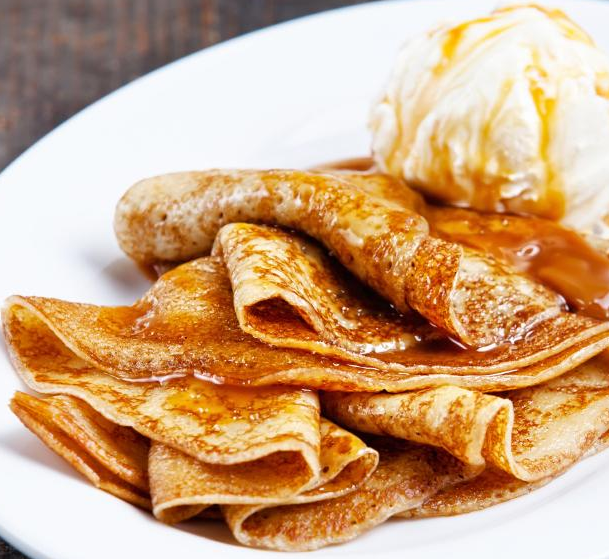
\includegraphics[width=0.25\textwidth]{panqueques}
    \introduction{
        Los panqueques se hacían en casa algunas veces, que buenos recuerdos que me traían de pequeño
        }
    \ingredients{
        1 & Taza y media de leche semidescremada \\
        2 & Huevos \\
        1 & Cucharada de aceite \\
        1 & Taza y media de harina cernida \\
        12 & Cucharadas de manjar \\
    }
    \preparation{
    \begin{enumerate}
            \item Junta todos los ingredientes en el jarro de una juguera vertiendo primero los líquidos como la leche, huevos y aceite y al final los secos (de este modo será más fácil integrar todo), menos el manjar. Procesa a velocidad media durante unos segundos hasta conseguir un batido homogéneo.
            \item Luego calienta una sartén de teflón o antiadherente de diametro mediano, vierte ¾ de un cucharón y distribuye por toda la sartén con movimientos circulares e inclinados con el mango de la sartén. Cocina durante unos segundos hasta dorar sus bordes y voltea. 
            \item Cocina unos segundos mas y repite el procedimiento hasta acabar la mezcla.
            \item Una vez listos, rellénalos uno a uno con una cucharada de manjar  y enróllalos sobre sí mismos, espolvorea azúcar flor y sírvelos de inmediato fríos o calientes como más te guste.
     \end{enumerate}
    }
\end{recipe}

% Tragos
\chapter*{Tragos Y Cócteles}
\addcontentsline{toc}{chapter}{Tragos Y Cócteles}

%Café
\chapter*{Café}
\addcontentsline{toc}{chapter}{Café}
% Recetas de Cafés
\newpage
Hay muchas maneras de preparar el café, dependiendo del tipo de grano entre otras cosas se puede apreciar de diversas profundidades de sabores, acidez, aromas...

Sin embargo, supongo que cada persona tendrá su preferencia en esto último, y disfrutar según las típicas recetas tradicionales...

\begin{center}
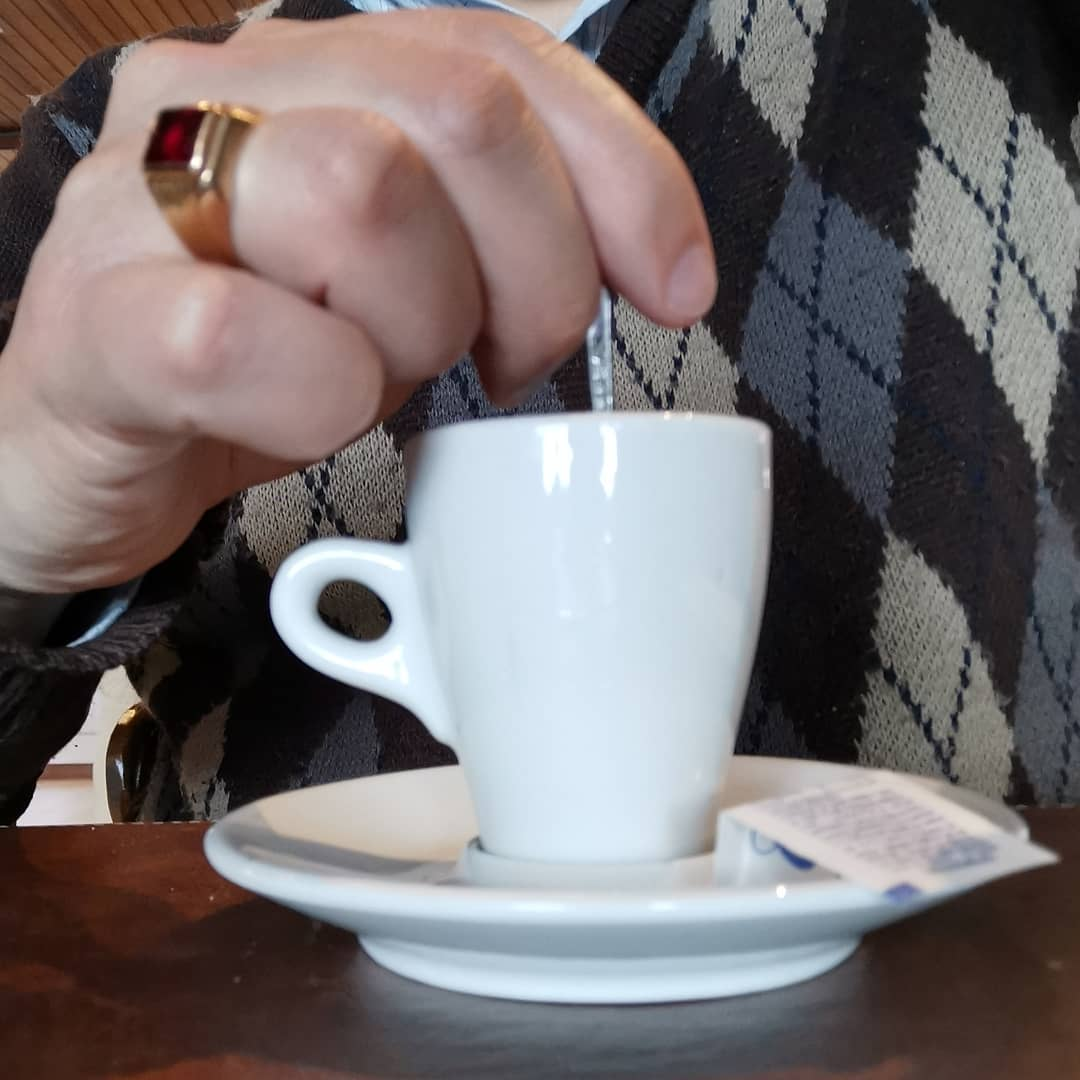
\includegraphics[scale=0.25]{cover_cafe}
\end{center}

\newpage
% Café Irlandés
\begin{recipe}[source={Barista de IG}]{Café Irlandés}
	\introduction{
		El café irlandés es un café muy rico para disfrutar sobre todo en clímas fríos. La primera vez que lo probé fue en Concepción en el café Cantabria.
	}
	\ingredients{
		\unit[1]{oz} & de almibar de canela \\
		\unit[2]{oz} & de whisky \\
        \unit[3]{oz} & de café \\
        \unit[1.5]{oz} & de crema de leche líquida
	}
	\preparation{
		\begin{enumerate}
			\item Agregar agua hirviendo a una taza para que adquiera la temperatura, y luego de unos segundos, retirar.
			\item Agregar el almibar.
			\item Agregar el whisky.
			\item Agregar el café.
			\item En una coctelera, batir por 10 segundos la crema de leche.
			\item Con ayuda de la cuchara, agregar lentamente la crema de leche en la taza.
			\item Para finalizar, se puede empolvorear con canela (opcional).
		\end{enumerate}
	}
\end{recipe}

\end{document}